\section{已有方法的解决方案与可迁移设计}
\subsection{FACET 的动态参考与 teacher--student}
FACET 用虚拟动力学生成 CoM 参考轨迹，其核心形式为
\begin{equation}
 m\ddot{\bm x}_{\rm ref}=K_p(\bm x_{\rm des}-\bm x_{\rm ref})
 +K_d(\dot{\bm x}_{\rm des}-\dot{\bm x}_{\rm ref})+\bm f_{\rm ext}.
\end{equation}
策略通过位置与速度跟踪奖励学习响应，并在多个时间起点生成的参考之间进行平滑。第一阶段用特权信息训练 teacher，同时用历史传感信息训练估计器预测特权特征。第二阶段以 teacher 初始化 student，并继续用 PPO 适应估计误差。论文中的估计器为隐藏维度 256 的 GRU，策略输出关节目标。该方法提供动态参考、参数条件化与隐状态估计的组合。\cite{facet2025}

迁移到当前冻结底座时，可以先把参考轨迹的速度分量变成底座命令，并测试底座的可跟踪范围。冻结底座的运动能力、时延和训练分布会限制可实现的虚拟动力学，直接替换参考公式的收益需要闭环验证。

\subsection{监督力估计与直接全身力控制}
Seeing-Eye 方法同时训练本体观测驱动的速度/外力估计器和 RL 行走策略。估计器使用仿真真值监督，估计力的方向进一步生成导航目标。迁移时可以增加
$L_F=\E\|\hat{\bm F}-\bm F_{\rm applied}\|^2$，再将估计力输入动态参考。这样可分别量化力估计误差和底座执行误差。\cite{defazio2023}

Portela 等的方法把末端力命令直接纳入任务，策略协调机械臂与腿。历史观测估计模块用监督损失学习特权状态，actor/critic 用 PPO 训练，奖励包含末端力、位置和机身运动项。该结构适合进一步扩展手腕交互，机器人模型、输出动作和训练环境都需支持机械臂。\cite{portela2024}

\subsection{显式导纳与运动 RL 的组合}
Schperberg 等使用腕部六维 F/T 传感器，将外部力旋量映射为末端速度，由机械臂与腿共同跟踪。其 Reference Governor 根据模型约束调整参考，状态估计采用神经网络增强的 Kalman filter。论文展示了 Go2 与六自由度机械臂上的交互。其约束保证依赖模型和假设，迁移时需重新建立对应的约束集合。\cite{schperberg2026}

对当前系统，有力传感器时可直接构造“测力、动态导纳、速度底座”的链路。无力传感器时可加入力估计器或特权特征蒸馏。若需要学习补偿，将修正写为
\begin{equation}
 \bm\delta_t=\bm\delta_{\rm adm,t}+\bm r_\theta(h_t,\bm c^0_t,\bm\delta_{\rm adm,t}),
\end{equation}
其中 $\bm r_\theta$ 有幅值约束，用来补偿底座跟踪和地形影响。Residual RL 的原始思想是叠加已有控制输出与学习残差，当前式子是针对速度命令层的设计提案。\cite{johannink2018}

\subsection{针对本仓库的动态参考方案}
下面给出一个可直接用来设计实验的参考更新式。对单轴 $m\dot\delta+d\delta=F$，假设一个周期内 $F$ 恒定，精确离散化为
\begin{equation}
 \delta_{k+1}=e^{-d\Delta t/m}\delta_k+
 \frac{1-e^{-d\Delta t/m}}{d}F_k.
\label{eq:exact}
\end{equation}
之后再施加运动能力对应的速度与变化率限制。若需要力死区，可使用连续函数
\begin{equation}
F_{\rm eff}=\sgn(F)\max(|F|-F_0,0).
\end{equation}
在旋转轴将 $F,m,d$ 分别换为 $\tau_z,J_z,d_\psi$。

取 $m=10\,\mathrm{kg}$、$d=20\,\mathrm{N\,s/m}$、$\Delta t=0.02\,\mathrm s$，持续 $20\,\mathrm N$ 拉力的稳态修正为 $1\,\mathrm{m/s}$，时间常数为 $0.5\,\mathrm s$，从静止开始的第一步约为 $0.0392\,\mathrm{m/s}$。松手后每步乘以 $e^{-0.04}$，形成可解释的衰减过程。该数值例子用于解释模型，实际虚拟参数需按底座能力与评价结果选择。

\begin{figure}[htbp]\centering
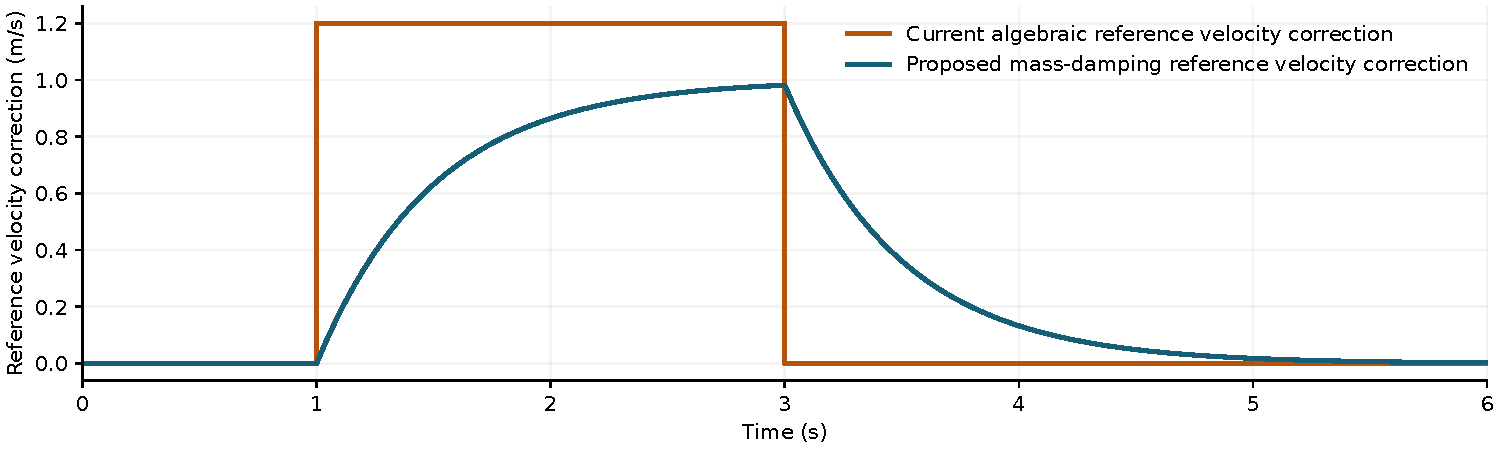
\includegraphics[width=\linewidth]{figures/reference_dynamics.pdf}
\caption{解析示例。$1\le t<3\,\mathrm s$ 时施加 $20\,\mathrm N$，其余时间为零。当前参考即时切换，质量--阻尼参考按式~\eqref{eq:exact} 演化。曲线为参考模型计算结果。}
\end{figure}

实施时可依次完成三个可独立验收的实验。首先对齐已施加力与观测时间戳，用同一参考、同一数据预算比较 MSE 和 PPO。然后用动态参考替换当前代数映射，检查力幅值响应及松手衰减。最后将 $\bm M,\bm D$ 作为输入，并在训练中随机采样参数，比较显式测力、监督力估计和 GRU 特征估计三种传感条件。完整关节级 teacher--student 与冻结底座方案分别报告结果，保持任务能力的可比性。
